\documentclass[./standalone.tex]{subfiles}
%\documentclass[../../../CR/pac.tex]{subfiles}

\begin{document}

\chapter{Génération des index}

\section{Index hiérarchiques}

\subsection{Définition}
Un index hiérarchique ou arborescent est une forme d'indexation où les entrées sont contenues dans d'autres entrées, etc. reflétant ainsi la généralisation (on remonte dans l'arbre) ou la spécification (on descend dans l'arbre) des entrées les unes par rapport aux autres.\\

Ce type d'index est appelé \textit{indexT} dans le code en référance à l'anglais \textit{\textbf{T}ree Index}.\\

\begin{figure}[h!]
    \centering
    \includegraphics[scale=0.425]{images/2_specFonc/index/indexHierarchique.png}
    \caption{Exemple d'indexation hiérarchique}
    \label{fig:indexT}
\end{figure}

\newpage
\subsection{Solution 1}
\bigskip
\bigskip
\subsubsection{Description de l'algorithme\\}
\paragraph{Étape 1\\\\}
On tronque de la liste des chemins récoltés la partie correspondant à la racine où est effectué l'index et on en profite pour mettre les chemins tronqués dans un tableau de chaînes de caractères.\\

\begin{center}
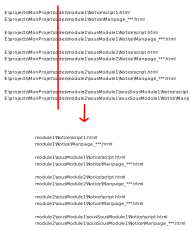
\includegraphics[scale=0.6]{images/2_specFonc/index/indexT_algo1_etape1.png}
\captionof{figure}{Suppression de la partie commune inutile}
\label{fig:indexT_algo1_etape1}
\end{center}

\newpage
\paragraph{Étape 2\\\\}
Si le paramètre \textit{isExhaustive} est à \textit{false} on supprime également de l'indexation les entrées qui ne sont pas des pages de manuel comme illustré ici:\\
\begin{center}
	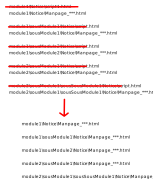
\includegraphics[scale=0.6]{images/2_specFonc/index/indexT_algo1_etape2.png}
	\captionof{figure}{Suppression des entrées qui ne sont pas des pages de manuel}
	\label{fig:indexT_algo1_etape2}
\end{center}

\newpage
\paragraph{Étape 3\\\\}
Chaque chemin absolu est ensuite traité par la méthode \textit{globalIndexArrMake(obj, subpathsList)} qui se charge d'en faire un tableau de noeuds\footnote{Une structure de donnée serait probablement plus appropriée ici...}. Les chemins absolus sont reconstitués en reconcaténant la partie tronquée à l'étape 1.
\begin{center}
	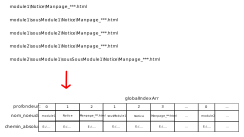
\includegraphics[scale=0.65]{images/2_specFonc/index/indexT_algo1_etape3.png}
	\captionof{figure}{Transformation des chaînes de caractères en tableaux de noeuds}
	\label{fig:indexT_algo1_etape2}
\end{center}

\paragraph{Étape 4\\\\}

\paragraph{Bilan\\\\}


\end{document}